\subsection{Implementation Complexity}
\begin{frame}{\subsecname}
	Frage:
	\begin{itemize}
		\item Wie groß ist der Aufwand das Scheduling-Verfahren zu implementieren?
	\end{itemize}
	Antwort:
	\begin{itemize}
		\item Rate Monotonics ist einfacher zu implementieren!
	\end{itemize}
\end{frame}

\begin{frame}{\subsecname}
	Ist es so einfach?\\\pause
	Faktoren:
	\begin{itemize}
		\item Wird auf einem bestehenden System entwickelt?
		\item Sind die Prioritäten festgesetzt oder können diese während der Laufzeit verändert werden?
		\item Wie viele Prioritäts-Level gibt es? %TODO Beispiel?
	\end{itemize}
\end{frame}

\begin{frame}{\subsecname}
	Annahme
	\begin{itemize}
		\item Das System wird von Grund auf mit einer Ready-Qeue implementiert\pause
		\item In dieser werden die Tasks für Rate Monotonics
			\begin{itemize}
				\item absteigend nach nach den Proritäten-Leveln
			\end{itemize}
			und für Erliest Deadline First
			\begin{itemize}
				\item aufsteigend nach der absoluten Deadline
			\end{itemize} gespeichert.
	\end{itemize}
\end{frame}

\subsection{Runtime Overhead}
\begin{frame}{\subsecname}
	Vorurteil:
	\begin{itemize}
		\item Rate Monotonics produziert weniger Runtime-Overhead, da die Prioritäten währen der Laufzeit nicht neu berechnet werden müssen
	\end{itemize}
\end{frame}

\newcommand{\showRMSlideRO}[1] {\begin{frame}{Beispiel Rate Monotonics}
	\begin{center}
		%\rowcolors{1}{RoyalBlue!20}{RoyalBlue!5}
		\begin{tabular}{c||c|c}
			Task ($\uptau_i$) & Dauer ($C_i$) & Task-Periode ($T_i$)\\\hline\hline
			$\uptau_1$ & 4 & 10\\
			$\uptau_2$ & 8 & 14
		\end{tabular}
	\end{center}
	\input{graphics/vergleich/runtimeOverhead#1_RM.tex}
\end{frame}}

\forloop{ct}{1}{\value{ct} < 8}%
{%
	\showRMSlideRO{\arabic{ct}}
}


\begin{frame}{Beispiel Erliest Deadline First}
	\begin{center}
		%\rowcolors{1}{RoyalBlue!20}{RoyalBlue!5}
		\begin{tabular}{c||c|c}
			Task ($\uptau_i$) & Dauer ($C_i$) & Task-Periode ($T_i$)\\\hline\hline
			$\uptau_1$ & 4 & 10\\
			$\uptau_2$ & 8 & 14
		\end{tabular}
	\end{center}
	\begin{figure}[htbp]
	% Partly taken from http://www.texample.net/tikz/examples/convolution-of-two-functions/
	\centering
	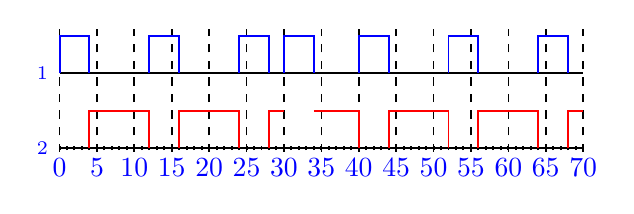
\begin{tikzpicture}[
		scale=0.095,
		line width=0.25mm,
		every node/.style={scale=1, text=blue},
		major tick/.style={semithick, dashed},
		x tick label/.style={anchor=north, minimum width=5mm},
		task1/.style={blue},
		task2/.style={red},
		task3/.style={green},
		desc/.style={anchor=east}
		]
	
	% Task 2
	\draw (0, 0) -- (70, 0);
	\node[desc] at (0, 0) {$\uptau_2$};
	
	% Task 1
	\draw (0, 10) -- (70, 10);
	\node[desc] at (0, 10) {$\uptau_1$};	
	
	% Small ticks
	\foreach \x in {0, 1,...,70}{
		\draw (\x, -0.25) -- (\x, 0.25);
	}
	
	% Major ticks with label
	\foreach \x/\label in {0, 5,...,70}{
		\node[x tick label] at (\x, 0) {$\label$}; 		
		\draw[major tick] (\x, -0.5) -- (\x, 16);
	}
	
	% Draw all
%	\foreach \x in {0, 10,...,69}{
%		\draw[task1] (\x, 10) -- (\x, 15) -- (\x+4, 15) -- (\x+4, 10);
%	}

	\draw[task1] (0, 10) --  (0, 15) --  (4, 15) -- (4, 10);
	\draw[task2] (4, 0) --  (4, 5) --  (12, 5) -- (12, 0);
	\draw[task1] (12, 10) --  (12, 15) --  (16, 15) -- (16, 10);
	\draw[task2] (16, 0) --  (16, 5) --  (24, 5) -- (24, 0);
	\draw[task1] (24, 10) --  (24, 15) --  (28, 15) -- (28, 10);
	\draw[task2] (28, 0) --  (28, 5) --  (30, 5); % 2 done
	\draw[task1] (30, 10) --  (30, 15) --  (34, 15) -- (34, 10);
	\draw[task2] (34, 5) --  (40, 5) -- (40, 0);	
	\draw[task1] (40, 10) --  (40, 15) --  (44, 15) -- (44, 10);
	\draw[task2] (44, 0) --  (44, 5) --  (52, 5) -- (52, 0);
	\draw[task1] (52, 10) --  (52, 15) --  (56, 15) -- (56, 10);
	\draw[task2] (56, 0) --  (56, 5) --  (64, 5) -- (64, 0);
	\draw[task1] (64, 10) --  (64, 15) --  (68, 15) -- (68, 10);
	\draw[task2] (68, 0) --  (68, 5) --  (70, 5);
		
	\end{tikzpicture}
%	\caption{Ablaufübersicht}
\end{figure} 
\end{frame}

\begin{frame}{\subsecname}
	Aber:\pause
	\begin{itemize}
		\item Zieht man den Aufwand der Context-Switches in Betracht ergibt sich ein anderes Bild
	\end{itemize}
\end{frame}

\begin{frame}{\subsecname}
	Context-Switching/Preemptions:
	\begin{itemize}
		\item Umschalten zwischen verschiedenen Tasks
		\item Zieht Aufwände mit sich
	\end{itemize}
\end{frame}

\begin{frame}{\subsecname}
	Rate Monotonics:
	\begin{figure}[htbp]
	% Partly taken from http://www.texample.net/tikz/examples/convolution-of-two-functions/
	\centering
	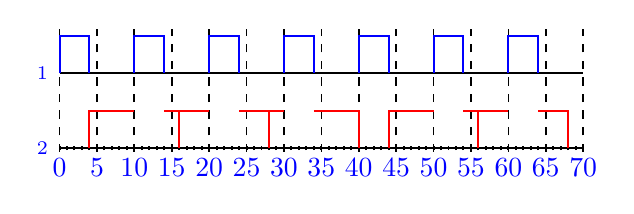
\begin{tikzpicture}[
		scale=0.095,
		line width=0.25mm,
		every node/.style={scale=1, text=blue},
		major tick/.style={semithick, dashed},
		x tick label/.style={anchor=north, minimum width=5mm},
		task1/.style={blue},
		task2/.style={red},
		task3/.style={green},
		desc/.style={anchor=east}
		]
	
	% Task 2
	\draw (0, 0) -- (70, 0);
	\node[desc] at (0, 0) {$\uptau_2$};
	
	% Task 1
	\draw (0, 10) -- (70, 10);
	\node[desc] at (0, 10) {$\uptau_1$};	
	
	% Small ticks
	\foreach \x in {0, 1,...,70}{
		\draw (\x, -0.25) -- (\x, 0.25);
	}
	
	% Major ticks with label
	\foreach \x/\label in {0, 5,...,70}{
		\node[x tick label] at (\x, 0) {$\label$}; 		
		\draw[major tick] (\x, -0.5) -- (\x, 16);
	}
	
	% Draw all
%	\foreach \x in {0, 10,...,69}{
%		\draw[task1] (\x, 10) -- (\x, 15) -- (\x+4, 15) -- (\x+4, 10);
%	}

	\draw[task1] (0, 10) --  (0, 15) --  (4, 15) -- (4, 10);	
	\draw[task2] (4, 0) -- (4, 5) -- (10, 5);
	\draw[task1] (10, 10) -- (10, 15) -- (14, 15) -- (14, 10);
	\draw[task2] (14, 5) -- (16, 5) -- (16, 0);
	\draw[task2] (16, 0) -- (16, 5) -- (20, 5);
	\draw[task1] (20, 10) -- (20, 15) -- (24, 15) -- (24, 10);
	\draw[task2] (24, 5) -- (28, 5) -- (28, 0);
	\draw[task2] (28, 0) -- (28, 5) -- (30, 5);
	\draw[task1] (30, 10) -- (30, 15) -- (34, 15) -- (34, 10);
	\draw[task2] (34, 5) -- (40, 5) -- (40, 0);
	\draw[task1] (40, 10) -- (40, 15) -- (44, 15) -- (44, 10);
	\draw[task2] (44, 0) -- (44, 5) -- (50, 5);
	\draw[task1] (50, 10) -- (50, 15) -- (54, 15) -- (54, 10);
	\draw[task2] (54, 5) -- (56, 5) -- (56, 0);
	\draw[task2] (56, 0) -- (56, 5) -- (60, 5);
	\draw[task1] (60, 10) -- (60, 15) -- (64, 15) -- (64, 10);
	\draw[task2] (64, 5) -- (68, 5) -- (68, 0);
		
	\end{tikzpicture}
%	\caption{Ablaufübersicht}
\end{figure} 
	Erliest Deadline First:
	\begin{figure}[htbp]
	% Partly taken from http://www.texample.net/tikz/examples/convolution-of-two-functions/
	\centering
	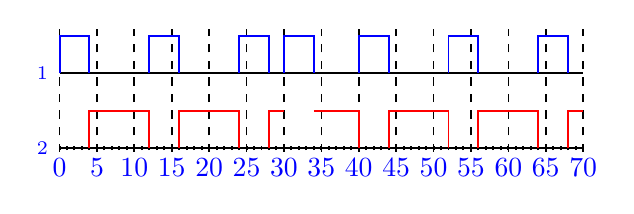
\begin{tikzpicture}[
		scale=0.095,
		line width=0.25mm,
		every node/.style={scale=1, text=blue},
		major tick/.style={semithick, dashed},
		x tick label/.style={anchor=north, minimum width=5mm},
		task1/.style={blue},
		task2/.style={red},
		task3/.style={green},
		desc/.style={anchor=east}
		]
	
	% Task 2
	\draw (0, 0) -- (70, 0);
	\node[desc] at (0, 0) {$\uptau_2$};
	
	% Task 1
	\draw (0, 10) -- (70, 10);
	\node[desc] at (0, 10) {$\uptau_1$};	
	
	% Small ticks
	\foreach \x in {0, 1,...,70}{
		\draw (\x, -0.25) -- (\x, 0.25);
	}
	
	% Major ticks with label
	\foreach \x/\label in {0, 5,...,70}{
		\node[x tick label] at (\x, 0) {$\label$}; 		
		\draw[major tick] (\x, -0.5) -- (\x, 16);
	}
	
	% Draw all
%	\foreach \x in {0, 10,...,69}{
%		\draw[task1] (\x, 10) -- (\x, 15) -- (\x+4, 15) -- (\x+4, 10);
%	}

	\draw[task1] (0, 10) --  (0, 15) --  (4, 15) -- (4, 10);
	\draw[task2] (4, 0) --  (4, 5) --  (12, 5) -- (12, 0);
	\draw[task1] (12, 10) --  (12, 15) --  (16, 15) -- (16, 10);
	\draw[task2] (16, 0) --  (16, 5) --  (24, 5) -- (24, 0);
	\draw[task1] (24, 10) --  (24, 15) --  (28, 15) -- (28, 10);
	\draw[task2] (28, 0) --  (28, 5) --  (30, 5); % 2 done
	\draw[task1] (30, 10) --  (30, 15) --  (34, 15) -- (34, 10);
	\draw[task2] (34, 5) --  (40, 5) -- (40, 0);	
	\draw[task1] (40, 10) --  (40, 15) --  (44, 15) -- (44, 10);
	\draw[task2] (44, 0) --  (44, 5) --  (52, 5) -- (52, 0);
	\draw[task1] (52, 10) --  (52, 15) --  (56, 15) -- (56, 10);
	\draw[task2] (56, 0) --  (56, 5) --  (64, 5) -- (64, 0);
	\draw[task1] (64, 10) --  (64, 15) --  (68, 15) -- (68, 10);
	\draw[task2] (68, 0) --  (68, 5) --  (70, 5);
		
	\end{tikzpicture}
%	\caption{Ablaufübersicht}
\end{figure} 
\end{frame}

\begin{frame}{\subsecname}
	Rate Monotonics:
	\begin{figure}[htbp]
	% Partly taken from http://www.texample.net/tikz/examples/convolution-of-two-functions/
	\centering
	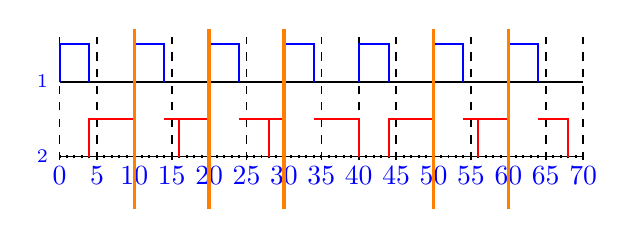
\begin{tikzpicture}[
		scale=0.095,
		line width=0.25mm,
		every node/.style={scale=1, text=blue},
		major tick/.style={semithick, dashed},
		x tick label/.style={anchor=north, minimum width=5mm},
		task1/.style={blue},
		task2/.style={red},
		task3/.style={green},
		desc/.style={anchor=east},
		konf/.style={orange, very thick}
		]
	
	% Task 2
	\draw (0, 0) -- (70, 0);
	\node[desc] at (0, 0) {$\uptau_2$};
	
	% Task 1
	\draw (0, 10) -- (70, 10);
	\node[desc] at (0, 10) {$\uptau_1$};	
	
	% Small ticks
	\foreach \x in {0, 1,...,70}{
		\draw (\x, -0.25) -- (\x, 0.25);
	}
	
	% Major ticks with label
	\foreach \x/\label in {0, 5,...,70}{
		\node[x tick label] at (\x, 0) {$\label$}; 		
		\draw[major tick] (\x, -0.5) -- (\x, 16);
	}
	
	% Draw all
%	\foreach \x in {0, 10,...,69}{
%		\draw[task1] (\x, 10) -- (\x, 15) -- (\x+4, 15) -- (\x+4, 10);
%	}

	\draw[task1] (0, 10) --  (0, 15) --  (4, 15) -- (4, 10);	
	\draw[task2] (4, 0) -- (4, 5) -- (10, 5);
	\draw[task1] (10, 10) -- (10, 15) -- (14, 15) -- (14, 10);
	\draw[task2] (14, 5) -- (16, 5) -- (16, 0);
	\draw[task2] (16, 0) -- (16, 5) -- (20, 5);
	\draw[task1] (20, 10) -- (20, 15) -- (24, 15) -- (24, 10);
	\draw[task2] (24, 5) -- (28, 5) -- (28, 0);
	\draw[task2] (28, 0) -- (28, 5) -- (30, 5);
	\draw[task1] (30, 10) -- (30, 15) -- (34, 15) -- (34, 10);
	\draw[task2] (34, 5) -- (40, 5) -- (40, 0);
	\draw[task1] (40, 10) -- (40, 15) -- (44, 15) -- (44, 10);
	\draw[task2] (44, 0) -- (44, 5) -- (50, 5);
	\draw[task1] (50, 10) -- (50, 15) -- (54, 15) -- (54, 10);
	\draw[task2] (54, 5) -- (56, 5) -- (56, 0);
	\draw[task2] (56, 0) -- (56, 5) -- (60, 5);
	\draw[task1] (60, 10) -- (60, 15) -- (64, 15) -- (64, 10);
	\draw[task2] (64, 5) -- (68, 5) -- (68, 0);
	
	\draw[konf] (10, 17) -- (10, -7);
	\draw[konf] (20, 17) -- (20, -7);
	\draw[konf] (30, 17) -- (30, -7);
	\draw[konf] (50, 17) -- (50, -7);
	\draw[konf] (60, 17) -- (60, -7);
		
	\end{tikzpicture}
%	\caption{Ablaufübersicht}
\end{figure} 
	Erliest Deadline First:
	\begin{figure}[htbp]
	% Partly taken from http://www.texample.net/tikz/examples/convolution-of-two-functions/
	\centering
	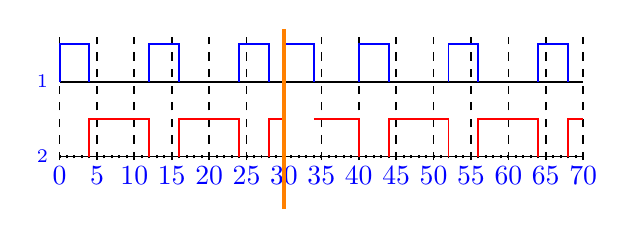
\begin{tikzpicture}[
		scale=0.095,
		line width=0.25mm,
		every node/.style={scale=1, text=blue},
		major tick/.style={semithick, dashed},
		x tick label/.style={anchor=north, minimum width=5mm},
		task1/.style={blue},
		task2/.style={red},
		task3/.style={green},
		desc/.style={anchor=east},
		konf/.style={orange, very thick}
		]
	
	% Task 2
	\draw (0, 0) -- (70, 0);
	\node[desc] at (0, 0) {$\uptau_2$};
	
	% Task 1
	\draw (0, 10) -- (70, 10);
	\node[desc] at (0, 10) {$\uptau_1$};	
	
	% Small ticks
	\foreach \x in {0, 1,...,70}{
		\draw (\x, -0.25) -- (\x, 0.25);
	}
	
	% Major ticks with label
	\foreach \x/\label in {0, 5,...,70}{
		\node[x tick label] at (\x, 0) {$\label$}; 		
		\draw[major tick] (\x, -0.5) -- (\x, 16);
	}
	
	% Draw all
%	\foreach \x in {0, 10,...,69}{
%		\draw[task1] (\x, 10) -- (\x, 15) -- (\x+4, 15) -- (\x+4, 10);
%	}

	\draw[task1] (0, 10) --  (0, 15) --  (4, 15) -- (4, 10);
	\draw[task2] (4, 0) --  (4, 5) --  (12, 5) -- (12, 0);
	\draw[task1] (12, 10) --  (12, 15) --  (16, 15) -- (16, 10);
	\draw[task2] (16, 0) --  (16, 5) --  (24, 5) -- (24, 0);
	\draw[task1] (24, 10) --  (24, 15) --  (28, 15) -- (28, 10);
	\draw[task2] (28, 0) --  (28, 5) --  (30, 5); % 2 done
	\draw[task1] (30, 10) --  (30, 15) --  (34, 15) -- (34, 10);
	\draw[task2] (34, 5) --  (40, 5) -- (40, 0);	
	\draw[task1] (40, 10) --  (40, 15) --  (44, 15) -- (44, 10);
	\draw[task2] (44, 0) --  (44, 5) --  (52, 5) -- (52, 0);
	\draw[task1] (52, 10) --  (52, 15) --  (56, 15) -- (56, 10);
	\draw[task2] (56, 0) --  (56, 5) --  (64, 5) -- (64, 0);
	\draw[task1] (64, 10) --  (64, 15) --  (68, 15) -- (68, 10);
	\draw[task2] (68, 0) --  (68, 5) --  (70, 5);
	
	\draw[konf] (30, 17) -- (30, -7);	
	
	\end{tikzpicture}
%	\caption{Ablaufübersicht}
\end{figure} 
\end{frame}

\begin{frame}{\subsecname}
	Fazit:
	\begin{itemize}
		\item Beachtet man den Aufwand der Context-Switches, erzeugt Rate Monotonics mehr Overhead als Erliest Deadline First
	\end{itemize}
\end{frame}


\subsection{Schedulability Analysis}
\begin{frame}{\subsecname}
	Schedulability meint, dass eine Menge von periodischen Task mithilfe eines Algorithmus planbar ist.\\
	
	Vorurteil:
	\begin{itemize}
		\item Die Einteilung ist Rate Monotonics leichter berechenbar als bei Erliest Deadline First.
	\end{itemize}
\end{frame}

\begin{frame}{\subsecname}
	Allgemein:
	\begin{equation}
		U_i = C_i / T_i
	\end{equation}
	\begin{equation}
		U_P = \sum_{i=1}^n U_i
	\end{equation}
	Desweiteren gilt, dass ein Task-Set $P$ nur planbar seien kann, wenn
	\begin{equation}
		U_P \leq 1
	\end{equation}
\end{frame}

\begin{frame}{\subsecname}
	Beispiel:
	\begin{tabular}{c||c|c}
		Task ($\uptau_i$) & Dauer ($C_i$) & Task-Periode ($T_i$)\\\hline\hline
		$\uptau_1$ & 2 & 4\\
		$\uptau_2$ & 3 & 8\\
		$\uptau_3$ & 2 & 16
	\end{tabular}
	\begin{equation}
		U = \frac{1}{4} + \frac{3}{8} + \frac{2}{16} = \frac{12}{16} \leq 1
	\end{equation}
\end{frame}

\begin{frame}{\subsecname}
	Response Time Analysis (RTA) Algorithmus für Rate Monotonics:
	\begin{equation}
		D_i \geq
		\begin{cases}
   				R_i^{(0)}=C_i \\
   				R_i^{(k)}=C_i+ \sum_{j:D_j<D_i} \lceil \frac{R_i^{k-1}}{T_j}\rceil C_j
  		\end{cases}
	\end{equation}
	Processor Demand Criterion (PDC) Algorithmus für Erliest Deadline First:
	\begin{equation}
		\forall L > 0,\; \sum_{i=1}^n\lfloor \frac{L+T_i-D_i}{T_i}\rfloor C_i \leq L
	\end{equation}
\end{frame}

\begin{frame}
	\begin{center}
		
\includegraphics[width=0.7\textwidth]{graphics/memes/sciencedog.jpg}
	\end{center}
\end{frame}

\begin{frame}{\subsecname}
	\begin{center}
		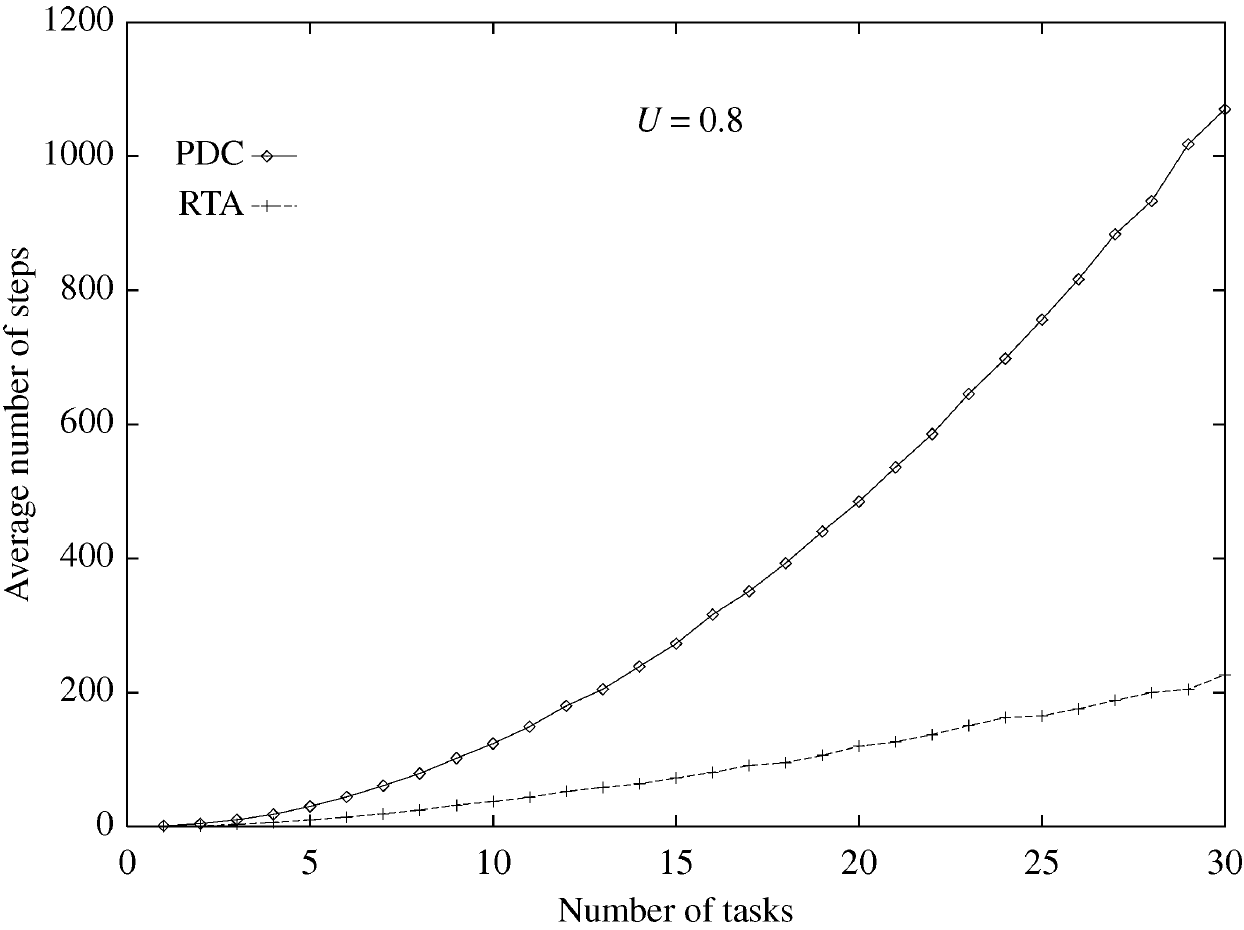
\includegraphics[scale=.25]{graphics/vergleich/rtapdc.png}	
	\end{center}
\end{frame}

\begin{frame}{\subsecname}
	Fazit:
	\begin{itemize}
		\item Komplexität für Rate Monotonics: pseudo-polynomial
		\item Komplexität für Erliest Deadline First:
		\begin{itemize}
			\item pseudo-polynomial
			\item in besonderen Fällen $O(n)$
		\end{itemize}
		\item Bei einer hohen Anzahl von Tasks ist Rate Monotonics besser zu berechnen (mit Ausnahmen)
	\end{itemize}
\end{frame}

\subsection{Robustness During Overloads}\label{RobustnessDuringOverloads}

\begin{frame}{\subsecname}
	Mythos:
	\begin{itemize}
		\item Rate Monotonics ist in Overload-Situationen besser vorhersehbar
	\end{itemize}$ $\\\pause
	Szenarien:
	\begin{itemize}
		\item Permanent Overload
		\item Transient Overload
	\end{itemize}
\end{frame}

\subsubsection{Permanent Overload}
\begin{frame}{Beispiel Rate Monotonics}
	\begin{center}
		\begin{tabular}{c||c|c}
			Task ($\uptau_i$) & Dauer ($C_i$) & Task-Periode ($T_i$)\\\hline\hline
			$\uptau_1$ & 4 & 8\\
			$\uptau_2$ & 6 & 12\\
			$\uptau_3$ & 5 & 20
		\end{tabular}
	\end{center}
	\begin{figure}[htbp]
	% Partly taken from http://www.texample.net/tikz/examples/convolution-of-two-functions/
	\centering
	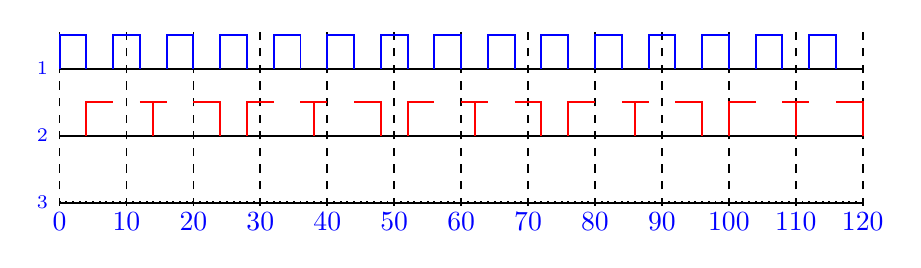
\begin{tikzpicture}[
		scale=0.085,
		line width=0.25mm,
		every node/.style={scale=1, text=blue},
		major tick/.style={semithick, dashed},
		x tick label/.style={anchor=north, minimum width=5mm},
		task1/.style={blue},
		task2/.style={red},
		task3/.style={green},
		desc/.style={anchor=east}
		]


	% Task 3
	\draw (0, 0) -- (120, 0);
	\node[desc] at (0, 0) {$\uptau_3$};
	
	% Task 2
	\draw (0, 10) -- (120, 10);
	\node[desc] at (0, 10) {$\uptau_2$};	

	% Task 1
	\draw (0, 20) -- (120, 20);
	\node[desc] at (0, 20) {$\uptau_1$};	

	
	% Small ticks
	\foreach \x in {0, 1,...,120}{
		\draw (\x, -0.25) -- (\x, 0.25);
	}
	
	% Major ticks with label
	\foreach \x/\label in {0, 10,...,120}{
		\node[x tick label] at (\x, 0) {$\label$}; 		
		\draw[major tick] (\x, -0.5) -- (\x, 26);
	}
	
	% Draw all
	\foreach \x in {0, 24,...,100}{
		\draw[task1] (\x, 20) -- (\x, 25) -- (\x+4, 25) -- (\x+4, 20);
		\draw[task2] (\x+4, 10) -- (\x+4, 15) -- (\x+8, 15);
		\draw[task1] (\x+8, 20) -- (\x+8, 25) -- (\x+12, 25) -- (\x+12, 20);
		\draw[task2] (\x+12, 15) -- (\x+14, 15) -- (\x+14, 10);
		\draw[task2] (\x+14, 10) -- (\x+14, 15) -- (\x+16, 15);
		\draw[task1] (\x+16, 20) -- (\x+16, 25) -- (\x+20, 25) -- (\x+20, 20);
		\draw[task2] (\x+20, 15) -- (\x+24, 15) -- (\x+24, 10);
	}

%	\draw[task1] (0, 10) --  (0, 15) --  (4, 15) -- (4, 10);	

		
	\end{tikzpicture}
%	\caption{Ablaufübersicht}
\end{figure} 
\end{frame}

\begin{frame}{Beispiel Erliest Deadline First}
	\begin{center}
		\begin{tabular}{c||c|c}
			Task ($\uptau_i$) & Dauer ($C_i$) & Task-Periode ($T_i$)\\\hline\hline
			$\uptau_1$ & 4 & 8\\
			$\uptau_2$ & 6 & 12\\
			$\uptau_3$ & 5 & 20
		\end{tabular}
	\end{center}
	\begin{figure}[htbp]
	% Partly taken from http://www.texample.net/tikz/examples/convolution-of-two-functions/
	\centering
	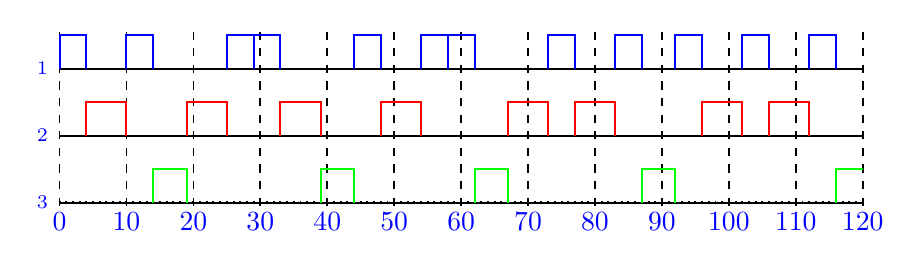
\begin{tikzpicture}[
		scale=0.085,
		line width=0.25mm,
		every node/.style={scale=1, text=blue},
		major tick/.style={semithick, dashed},
		x tick label/.style={anchor=north, minimum width=5mm},
		task1/.style={blue},
		task2/.style={red},
		task3/.style={green},
		desc/.style={anchor=east}
		]


	% Task 3
	\draw (0, 0) -- (120, 0);
	\node[desc] at (0, 0) {$\uptau_3$};
	
	% Task 2
	\draw (0, 10) -- (120, 10);
	\node[desc] at (0, 10) {$\uptau_2$};	

	% Task 1
	\draw (0, 20) -- (120, 20);
	\node[desc] at (0, 20) {$\uptau_1$};	

	
	% Small ticks
	\foreach \x in {0, 1,...,120}{
		\draw (\x, -0.25) -- (\x, 0.25);
	}
	
	% Major ticks with label
	\foreach \x/\label in {0, 10,...,120}{
		\node[x tick label] at (\x, 0) {$\label$}; 		
		\draw[major tick] (\x, -0.5) -- (\x, 26);
	}

	\draw[task1] (0, 20) --  (0, 25) --  (4, 25) -- (4, 20);
	\draw[task2] (4, 10) --  (4, 15) --  (10, 15) -- (10, 10);
	\draw[task1] (10, 20) --  (10, 25) --  (14, 25) -- (14, 20);
	\draw[task3] (14, 0) --  (14, 5) --  (19, 5) -- (19, 0);
	\draw[task2] (19, 10) --  (19, 15) --  (25, 15) -- (25, 10);
	\draw[task1] (25, 20) --  (25, 25) --  (29, 25) -- (29, 20);
	\draw[task1] (29, 20) --  (29, 25) --  (33, 25) -- (33, 20);
	\draw[task2] (33, 10) --  (33, 15) --  (39, 15) -- (39, 10);
	\draw[task3] (39, 0) --  (39, 5) --  (44, 5) -- (44, 0);
	\draw[task1] (44, 20) --  (44, 25) --  (48, 25) -- (48, 20);
	\draw[task2] (48, 10) --  (48, 15) --  (54, 15) -- (54, 10);
	\draw[task1] (54, 20) --  (54, 25) --  (58, 25) -- (58, 20);
	\draw[task1] (58, 20) --  (58, 25) --  (62, 25) -- (62, 20);
	\draw[task3] (62, 0) --  (62, 5) --  (67, 5) -- (67, 0);
	\draw[task2] (67, 10) --  (67, 15) --  (73, 15) -- (73, 10);
	\draw[task1] (73, 20) --  (73, 25) --  (77, 25) -- (77, 20);
	\draw[task2] (77, 10) --  (77, 15) --  (83, 15) -- (83, 10);
	\draw[task1] (83, 20) --  (83, 25) --  (87, 25) -- (87, 20);
	\draw[task3] (87, 0) --  (87, 5) --  (92, 5) -- (92, 0);
	\draw[task1] (92, 20) --  (92, 25) --  (96, 25) -- (96, 20);
	\draw[task2] (96, 10) --  (96, 15) --  (102, 15) -- (102, 10);
	\draw[task1] (102, 20) --  (102, 25) --  (106, 25) -- (106, 20);
	\draw[task2] (106, 10) --  (106, 15) --  (112, 15) -- (112, 10);
	\draw[task1] (112, 20) --  (112, 25) --  (116, 25) -- (116, 20);
	\draw[task3] (116, 0) --  (116, 5) --  (120, 5);
	
	\draw[task3] (14, 0) --  (14, 5) --  (19, 5) -- (19, 0);
		
	\end{tikzpicture}
%	\caption{Ablaufübersicht}
\end{figure} 
\end{frame}

\begin{frame}{Beispiel}
	\begin{figure}[htbp]
	% Partly taken from http://www.texample.net/tikz/examples/convolution-of-two-functions/
	\centering
	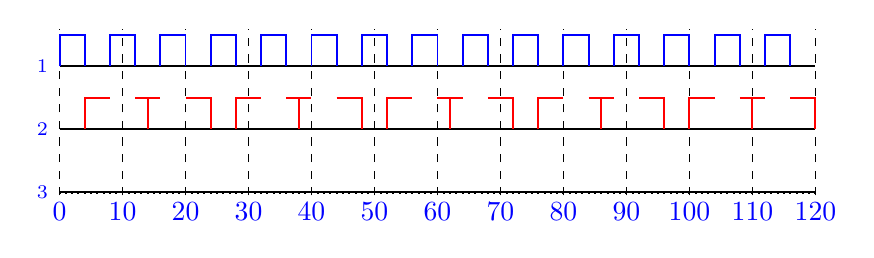
\begin{tikzpicture}[
		scale=0.08,
		line width=0.25mm,
		every node/.style={scale=1, text=blue},
		major tick/.style={semithick, dashed},
		x tick label/.style={anchor=north, minimum width=5mm},
		task1/.style={blue},
		task2/.style={red},
		task3/.style={green},
		desc/.style={anchor=east}
		]


	% Task 3
	\draw (0, 0) -- (120, 0);
	\node[desc] at (0, 0) {$\uptau_3$};
	
	% Task 2
	\draw (0, 10) -- (120, 10);
	\node[desc] at (0, 10) {$\uptau_2$};	

	% Task 1
	\draw (0, 20) -- (120, 20);
	\node[desc] at (0, 20) {$\uptau_1$};	

	
	% Small ticks
	\foreach \x in {0, 1,...,120}{
		\draw (\x, -0.25) -- (\x, 0.25);
	}
	
	% Major ticks with label
	\foreach \x/\label in {0, 10,...,120}{
		\node[x tick label] at (\x, 0) {$\label$}; 		
		\draw[major tick] (\x, -0.5) -- (\x, 26);
	}
	
	% Draw all
	\foreach \x in {0, 24,...,100}{
		\draw[task1] (\x, 20) -- (\x, 25) -- (\x+4, 25) -- (\x+4, 20);
		\draw[task2] (\x+4, 10) -- (\x+4, 15) -- (\x+8, 15);
		\draw[task1] (\x+8, 20) -- (\x+8, 25) -- (\x+12, 25) -- (\x+12, 20);
		\draw[task2] (\x+12, 15) -- (\x+14, 15) -- (\x+14, 10);
		\draw[task2] (\x+14, 10) -- (\x+14, 15) -- (\x+16, 15);
		\draw[task1] (\x+16, 20) -- (\x+16, 25) -- (\x+20, 25) -- (\x+20, 20);
		\draw[task2] (\x+20, 15) -- (\x+24, 15) -- (\x+24, 10);
	}

%	\draw[task1] (0, 10) --  (0, 15) --  (4, 15) -- (4, 10);	

		
	\end{tikzpicture}
%	\caption{Ablaufübersicht}
\end{figure} 
	\begin{figure}[htbp]
	% Partly taken from http://www.texample.net/tikz/examples/convolution-of-two-functions/
	\centering
	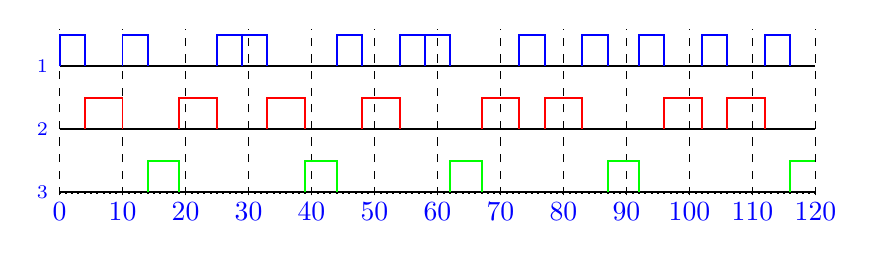
\begin{tikzpicture}[
		scale=0.08,
		line width=0.25mm,
		every node/.style={scale=1, text=blue},
		major tick/.style={semithick, dashed},
		x tick label/.style={anchor=north, minimum width=5mm},
		task1/.style={blue},
		task2/.style={red},
		task3/.style={green},
		desc/.style={anchor=east}
		]


	% Task 3
	\draw (0, 0) -- (120, 0);
	\node[desc] at (0, 0) {$\uptau_3$};
	
	% Task 2
	\draw (0, 10) -- (120, 10);
	\node[desc] at (0, 10) {$\uptau_2$};	

	% Task 1
	\draw (0, 20) -- (120, 20);
	\node[desc] at (0, 20) {$\uptau_1$};	

	
	% Small ticks
	\foreach \x in {0, 1,...,120}{
		\draw (\x, -0.25) -- (\x, 0.25);
	}
	
	% Major ticks with label
	\foreach \x/\label in {0, 10,...,120}{
		\node[x tick label] at (\x, 0) {$\label$}; 		
		\draw[major tick] (\x, -0.5) -- (\x, 26);
	}

	\draw[task1] (0, 20) --  (0, 25) --  (4, 25) -- (4, 20);
	\draw[task2] (4, 10) --  (4, 15) --  (10, 15) -- (10, 10);
	\draw[task1] (10, 20) --  (10, 25) --  (14, 25) -- (14, 20);
	\draw[task3] (14, 0) --  (14, 5) --  (19, 5) -- (19, 0);
	\draw[task2] (19, 10) --  (19, 15) --  (25, 15) -- (25, 10);
	\draw[task1] (25, 20) --  (25, 25) --  (29, 25) -- (29, 20);
	\draw[task1] (29, 20) --  (29, 25) --  (33, 25) -- (33, 20);
	\draw[task2] (33, 10) --  (33, 15) --  (39, 15) -- (39, 10);
	\draw[task3] (39, 0) --  (39, 5) --  (44, 5) -- (44, 0);
	\draw[task1] (44, 20) --  (44, 25) --  (48, 25) -- (48, 20);
	\draw[task2] (48, 10) --  (48, 15) --  (54, 15) -- (54, 10);
	\draw[task1] (54, 20) --  (54, 25) --  (58, 25) -- (58, 20);
	\draw[task1] (58, 20) --  (58, 25) --  (62, 25) -- (62, 20);
	\draw[task3] (62, 0) --  (62, 5) --  (67, 5) -- (67, 0);
	\draw[task2] (67, 10) --  (67, 15) --  (73, 15) -- (73, 10);
	\draw[task1] (73, 20) --  (73, 25) --  (77, 25) -- (77, 20);
	\draw[task2] (77, 10) --  (77, 15) --  (83, 15) -- (83, 10);
	\draw[task1] (83, 20) --  (83, 25) --  (87, 25) -- (87, 20);
	\draw[task3] (87, 0) --  (87, 5) --  (92, 5) -- (92, 0);
	\draw[task1] (92, 20) --  (92, 25) --  (96, 25) -- (96, 20);
	\draw[task2] (96, 10) --  (96, 15) --  (102, 15) -- (102, 10);
	\draw[task1] (102, 20) --  (102, 25) --  (106, 25) -- (106, 20);
	\draw[task2] (106, 10) --  (106, 15) --  (112, 15) -- (112, 10);
	\draw[task1] (112, 20) --  (112, 25) --  (116, 25) -- (116, 20);
	\draw[task3] (116, 0) --  (116, 5) --  (120, 5);
	
	\draw[task3] (14, 0) --  (14, 5) --  (19, 5) -- (19, 0);
		
	\end{tikzpicture}
%	\caption{Ablaufübersicht}
\end{figure} 
\end{frame}

\begin{frame}{\subsubsecname}
	\begin{columns}[]
  			\begin{column}{0.5\textwidth}
				Rate Monotonics:
				\begin{itemize}
					\item Tasks mit langer Periode werden vollständig blockiert!
					\item Gut vorhersagbar
				\end{itemize}

			\end{column}
  			\begin{column}{0.5\textwidth}
  				Erliest Deadline First:
				\begin{itemize}
					\item Sieht chaotischer aus
					\item Durchschnittliche Periode $\bar{T}_i$ für einen Task $\uptau_i$ ist gegeben durch
						\begin{equation}
							\bar{T}_i=T_i\cdot U
						\end{equation}
				\end{itemize}	
  			\end{column}
	\end{columns}
\end{frame}

%\begin{frame}{\subsubsecname}
%	Beispiel mit EDF? %TODO
%\end{frame}

\begin{frame}{\subsubsecname}
	Fazit:
	\begin{itemize}
		\item Beide Verfahren bei permanenter Überlastung sehr gut vorhersagbar
		\item Einsatzgebiet ist stark Situationsabhängig
	\end{itemize}
\end{frame}

\subsubsection{Transient Overload}
\begin{frame}{\subsubsecname}
	Annahme für RM:
	\begin{itemize}
		\item Es werden Tasks mit kurzen Perioden bevorzugt\pause
		\item[$\Rightarrow$] Falls ein Task seine Deadline überschreitet, wird der Task mit der längsten Periodenlänge verschoben/unterbrochen	
	\end{itemize}
\end{frame}

\newcommand{\showRMSlideRob}[1] {\begin{frame}{\subsubsecname}
	\begin{center}
		\begin{tabular}{c||c|c}
			Task ($\uptau_i$) & Dauer ($C_i$) & Task-Periode ($T_i$)\\\hline\hline
			$\uptau_1$ & 6 & 15\\
			$\uptau_2$ & 9 & 27\\
			$\uptau_3$ & 3 & 60\\
			$\uptau_4$ & 3 & 90
		\end{tabular}
	\end{center}
	\input{graphics/vergleich/transient#1_RM.tex}
\end{frame}}

\forloop{ct}{1}{\value{ct} < 8}%
{%
	\showRMSlideRob{\arabic{ct}}
}

\begin{frame}{\subsecname}
	Fazit:
	\begin{itemize}
		\item Permanent Overload: Gleichwertig
		\item Transient Overload:
		\begin{itemize}
			\item Rate Monotonics verführt zu falschen Annahmen
		\end{itemize}
	\end{itemize}
\end{frame}

\begin{frame}{\subsecname}
	\begin{center}
			
\includegraphics[scale=1]{graphics/memes/busted.jpg}
	\end{center}
\end{frame}

\subsection{Jitter and Latency}

\begin{frame}{\subsecname}
	Definition von Jitter:\\
	Absolute Response Time Jitter $ARJ_i$ ist definiert durch
	\begin{equation}
		ARJ_i=max R_{i,k}-min R_{i,k}
	\end{equation} mit
	$R_{i,K}$ als Response-Time für den $k$-ten Job von $\uptau_i$
\end{frame}

\begin{frame}{\subsecname}
	Vorurteil:
	\begin{itemize}
		\item Durch die festen Prioritäten entsteht währen der Laufzeit bei Rate Monotonics weniger Jitter als bei Erliest Deadline First. 
	\end{itemize}
\end{frame}

\newcommand{\showRMSlideJit}[1] {\begin{frame}{Beispiel Jitter Rate Monotonics}
		\begin{center}
		\begin{tabular}{c||c|c}
			Task ($\uptau_i$) & Dauer ($C_i$) & Task-Periode ($T_i$)\\\hline\hline
			$\uptau_1$ & 2 & 6\\
			$\uptau_2$ & 3 & 8\\
			$\uptau_3$ & 2 & 12
		\end{tabular}
	\end{center}
	\input{graphics/vergleich/jitter#1_RM.tex}
\end{frame}}

\forloop{ct}{1}{\value{ct} < 5}%
{%
	\showRMSlideJit{\arabic{ct}}
}

\begin{frame}{Beispiel Jitter Erliest Deadline First}
		\begin{center}
		\begin{tabular}{c||c|c}
			Task ($\uptau_i$) & Dauer ($C_i$) & Task-Periode ($T_i$)\\\hline\hline
			$\uptau_1$ & 2 & 6\\
			$\uptau_2$ & 3 & 8\\
			$\uptau_3$ & 2 & 12
		\end{tabular}
	\end{center}
	\begin{figure}[htbp]
	% Partly taken from http://www.texample.net/tikz/examples/convolution-of-two-functions/
	\centering
	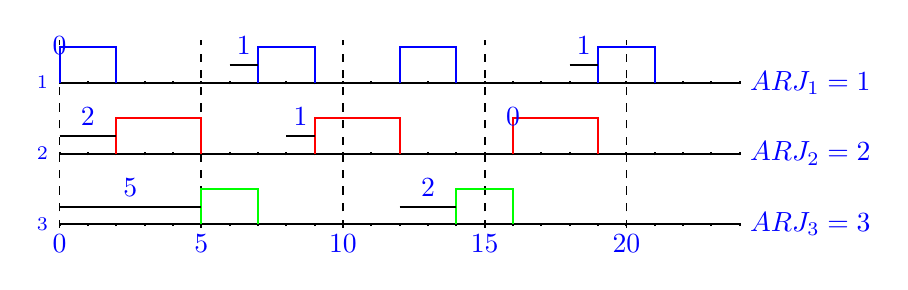
\begin{tikzpicture}[
		scale=0.09,
		line width=0.25mm,
		every node/.style={scale=1, text=blue},
		major tick/.style={semithick, dashed},
		x tick label/.style={anchor=north, minimum width=5mm},
		task1/.style={blue},
		task2/.style={red},
		task3/.style={green},
		desc/.style={anchor=east},
		arj/.style={anchor=west},
		desc2/.style={anchor=south}
		]

	% 24 96
	% Task 3
	\draw (0, 0) -- (96, 0);
	\node[desc] at (0, 0) {$\uptau_3$};
	
	% Task 2
	\draw (0, 10) -- (96, 10);
	\node[desc] at (0, 10) {$\uptau_2$};	

	% Task 1
	\draw (0, 20) -- (96, 20);
	\node[desc] at (0, 20) {$\uptau_1$};

	
	% Small ticks
	\foreach \x in {0, 4,...,96}{
		\draw (\x, -0.25) -- (\x, 0.25);
		\draw (\x, 19.75) -- (\x, 20.25);
		\draw (\x, 9.75) -- (\x, 10.25);
	}
	
	% Major ticks with label
	\foreach \x/\label in {0, 20,...,96}{		
		\draw[major tick] (\x, -0.5) -- (\x, 26);
	}
	
	\node[x tick label] at (0, 0) {0};
	\node[x tick label] at (20, 0) {5};
	\node[x tick label] at (40, 0) {10}; 
	\node[x tick label] at (60, 0) {15};
	\node[x tick label] at (80, 0) {20};
	
	% Draw all
	\draw[task1] (   0, 20) -- (   0, 25) -- ( 2*4, 25) -- ( 2*4, 20);
	\draw[task2] ( 2*4, 10) -- ( 2*4, 15) -- ( 5*4, 15) -- ( 5*4, 10);
	\draw[task3] ( 5*4,  0) -- ( 5*4,  5) -- ( 7*4,  5) -- ( 7*4,  0);
	\draw[task1] ( 7*4, 20) -- ( 7*4, 25) -- ( 9*4, 25) -- ( 9*4, 20);
	\draw[task2] ( 9*4, 10) -- ( 9*4, 15) -- (12*4, 15) -- (12*4, 10);
	\draw[task1] (12*4, 20) -- (12*4, 25) -- (14*4, 25) -- (14*4, 20);
	\draw[task3] (14*4,  0) -- (14*4,  5) -- (16*4,  5) -- (16*4,  0);
	\draw[task2] (16*4, 10) -- (16*4, 15) -- (19*4, 15) -- (19*4, 10);
	\draw[task1] (19*4, 20) -- (19*4, 25) -- (21*4, 25) -- (21*4, 20);

	% Task 1
	\node[desc2] at      (     0, 22.5) {0};
	\draw ( 6*4,22.5) -- (   7*4, 22.5);	
	\node[desc2] at      ( 6.5*4, 22.5) {1};
	\draw (18*4,22.5) -- (  19*4, 22.5);	
	\node[desc2] at      (18.5*4, 22.5) {1};
	\node[arj] at (96, 20)  {$ARJ_1=1$};
	
	% Task 2 ARJ
	\draw (   0,12.5) -- (  2*4, 12.5);
	\node[desc2] at      (  1*4, 12.5) {2};
	\draw ( 8*4,12.5) -- (  9*4, 12.5);
	\node[desc2] at      (8.5*4, 12.5) {1};
	\node[desc2] at      ( 16*4, 12.5) {0};
	\node[arj] at (96, 10) {$ARJ_2=2$};
	
	% Task 3 ARJ
	\draw (   0,2.5) -- (  5*4, 2.5);
	\node[desc2] at     (   10, 2.5) {5};
	\draw (12*4,2.5) -- ( 14*4, 2.5);
	\node[desc2] at     ( 13*4, 2.5) {2};
	\node[arj] at (96,  0) {$ARJ_3=3$};	

	\end{tikzpicture}
%	\caption{Ablaufübersicht}
\end{figure} 
\end{frame}

\begin{frame}{\subsecname}
	\begin{center}
		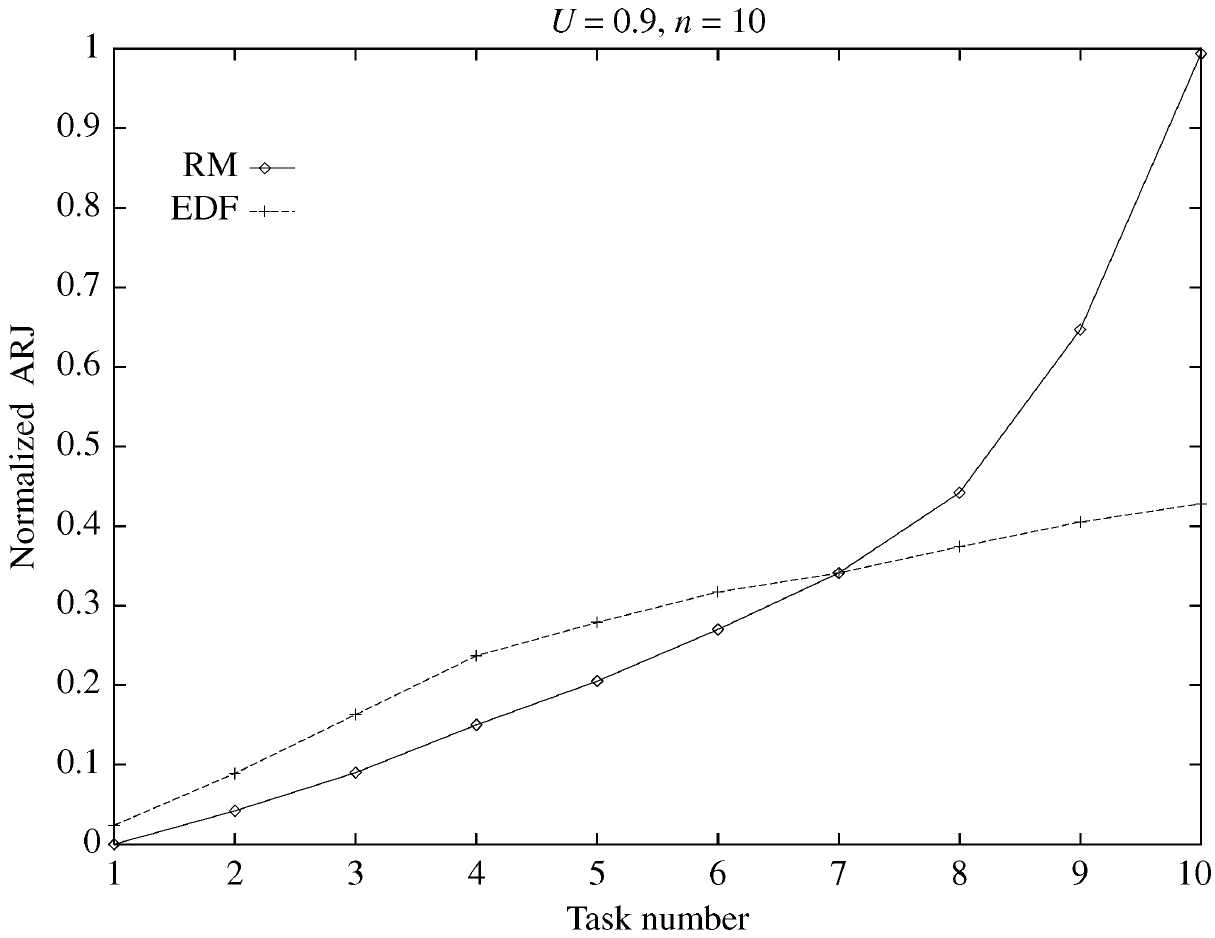
\includegraphics[scale=.25]{graphics/vergleich/jitter.png}	
	\end{center}
\end{frame}

\begin{frame}{\subsecname}
	Fazit:
	\begin{itemize}
		\item RM hält Jitter für die hoch priorisierten Tasks sehr niedrig, vernachlässigt jedoch die anderen Tasks
		\item Insgesamt erzeugt EDF, gerade bei hoher Auslastung, wesentlich weniger Jitter
	\end{itemize}
\end{frame}

%\subsection{Other Issues}
\subsubsection{Ressource Sharing}
\begin{frame}{\subsubsecname}
	Vorurteil:
	\begin{itemize}
		\item Es gibt nur für Rate Monotonics Protokolle um Zugriffe auf kritische Ressourcen zu regeln.
	\end{itemize}\pause
	Aber:
	\begin{itemize}
		\item Auch unter Erliest Deadline First gibt es diverse Algorithmen.
	\end{itemize}
\end{frame}

\subsubsection{Aperiodic Task Handling}
\begin{frame}{\subsubsecname}
	Test
\end{frame}

\subsubsection{Ressource Reservation}
\begin{frame}{\subsubsecname}
	Test
\end{frame}